\chapter{Génération de nombres premiers}

Dans cette section, on va se pencher sur la génération de nombre premier aléatoire. On va étudier 4 algorithmes: Algorithme \ref{Algorithme de recherche aléatoire}, Algorithme \ref{Algorithme de Gordon}, Algorithme \ref{Algorithme DSA}.
Ces algorithmes sont utilisés pour générer des grands nombres premiers pour le système RSA. 
Avec le développement d’internet, le besoin de transmettre des informations confidentielles de façon sécurisée est devenu primordial. C'est pour cela que de tels algorithmes existent car ils rendent la tâche aux adversaires plus difficile pour pouvoir déchiffrer une information.
La génération de nombre premier diffère des tests de primalités décrit à la section \ref{Test probabiliste de primalité} et \ref{Test de primalité} car ils permettent de générer un nombre premier non pas de savoir si un nombre est premier ou pas.

\section{Algorithme de recherche aléatoire}
Cet algorithme efficace va nous permettre de générer aléatoirement des nombres premiers d'une taille de bits passée en paramètre et d'un paramètre de sécurité. Il utilisera le test de Miller-Rabin qui est très efficace et qui nous permettra de générer un nombre premier probable notamment par des itérations du test.



\subsection{L'algorithme Random Search}
\label{Algorithme de recherche aléatoire}


\underline{Définition}:

Un \textbf{nombre premier probable} est un nombre qui a une certaine  probabilité d'être réellement premier. Il satisfait à une condition (nécessaire mais pas suffisante) qui est satisfaite aussi par tous les nombres premiers. 

\underline{\textbf{Algorithme Random Search}}:

\begin{algorithm}
\caption{RandomSearch($k$,$t$)}
\begin{algorithmic}[1]
\Require{Un entier $k$ le nombre de bits à générer pour $n$ et un paramètre de sécurité $t$}
\Ensure{un entier $n$ $k$-bit aléatoire probablement premier}
\State \textbf{Générer} un entier $n$ impair de $k$-bits aléatoirement
\State \textbf{Utiliser} la division successive pour déterminer si $n$ est divisible par n'importe quel entier impair premier $\leq B$ . Si oui revenir à la $1^{\text{ère}}$ étape.
\If{$MillerRabin(n,t)$ affiche $"premier"$} \Return "n" Sinon revenir à la $1^{\text{ère}}$ étape.
\EndIf
\end{algorithmic}
\end{algorithm}
Dans l'algorithme de recherche aléatoire, une stratégie raisonnable \label{raisonnable} pour sélectionner un nombre premier aléatoire de k bits (probable) est de sélectionner à plusieurs reprises des entiers impairs aléatoires de k bits de $n$ jusqu'à ce que l'on trouve un qui est déclaré "premier" par le test de $Miller Rabin(n,t)$ pour une valeur approprié du paramètre de sécurité t.

Tout d'abord, il faut vérifier que l'entier $n$ n'a pas de facteur premier. S'il est divisible par un petit nombre premier, il est moins coûteux d'exclure le candidat $n$ par division successive qu'en utilisant le test de Miller-Rabin.
Puisque la probabilité qu'un entier aléatoire $n$ ait un petit diviseur premier est relativement grande, avant d'appliquer le test de Miller-Rabin, le candidat $n$ doit être testé pour les petits diviseurs sous une borne $B$ prédéterminée. Cela peut être fait en divisant n par tous les nombres premiers inférieur à $B$.
On définit $B$ par la borne expérimentale. L'estimation du choix optimal pour B peut être obtenu expérimentalement.

\subsubsection{Espérance du nombre de génération aléatoire.}
Dans cette section on se donne pour objectif d’estimer le nombre de générations aléatoires dans l’algorithme RandomSearch.

\label{fait1}
\underline{\textbf{Proposition 1}} : Soit $\pi(x)$ représentant le nombre de nombres premiers $\leq x$. alors pour tout $x \geq 16$ 
$$\pi(x) > \dfrac{x}{\ln(x)}$$
$$\pi(x) < 1.25506\dfrac{x}{\ln(x)}$$
Soient $k>4$ le nombres de bits.
Comme le montre le Proposition 1, la proportion de nombres premiers est inférieure à $2^k$ et plus grande que $\frac{1}{k\ln(2)}$, en excluant les entier pairs, la proportion de nombres premiers impairs est inférieure à $2^k$ et supérieure à $\frac{2}{k\ln(2)}$. En particulier comme les nombres premiers sont relativement bien repartis on peut considérer que la probabilité qu’un nombre de $k$-bits impair tirée aléatoirement soit premier vaut $\frac{2}{k\ln(2)}$.

On considère ainsi tout naturellement l’expérience aléatoire consistant à générer un nombre aléatoire impair de $k$-bits et regarder si il est premier.

En notant $X$ la variable aléatoire comptant le nombre de génération aléatoire avant d’obtenir un nombre premier, $X$ suit une loi géométrique de paramètre $\frac{2}{k\ln(2)}$ de sorte que l’espérance de X vaut $\frac{k\ln(2)}{2}$.


Ainsi on va en moyenne générer $\frac{k\ln(2)}{2}$ nombres impairs aléatoires avant d’obtenir un nombre premier de $k$ bits ce qui explique en partie le coté "raisonnable" vu partie \ref{raisonnable} de l'algorithme RandomSearch.

\subsubsection{Résultats Expérimentaux}
Dans l'algorithme RandomSearch, la probabilité qu'un nombre de $k$-bits tiré aléatoirement soit facteur d'un petit nombre premier est relativement grande. En fait, si B est un entier positif, la proportion de nombres impairs divisibles par un nombre premier inférieur à B vaut $\prod_{3\leq p \leq B} \left(1-\frac{1}{p}\right)$.Ainsi dans l'algorithme RandomSearch, pour des raison d'efficacité, il est préconisé de tester le candidat $n$ pour des petits nombres premiers inférieurs à une borne B prédéterminé.

On se donne donc pour objectif d'estimer cette borne $B$ avec notre implémentation python à l'aide d'expérimentations.

Pour se faire, nous avons décider de tester le candidat $n$ à l’aide de l’opérateur modulo de python pour tous les nombres premier inférieur à $B$ pour $B \in \{0,4,8,16,32,64,128,256,512,1024,2048\}.$

Voici un tableau récapitulant la proportion d’entier éliminer pour chaque B et le nombres de nombre premier inférieur a B.


\begin{tabular}{|l|c|c|c|c|c|c|c|c|c|c|c|}
    \hline
    Borne B & 4 & 8 & 16 & 32 & 64 & 128 & 256 & 512 & 1024 & 2048 \\
    \hline
    Proportion de candidat éliminé  & 0,33 & 0,54 & 0,62 & 0,69 & 0,74 & 0,77 & 0,8 & 0,82 & 0,84 & 0,85 \\
    \hline
    Nombre de nombre premier < B & 1 & 3 & 5 & 10 & 17 & 30 & 53 & 96 & 171 & 308 \\
    \hline
\end{tabular}



\begin{figure}[H]
    \centering
    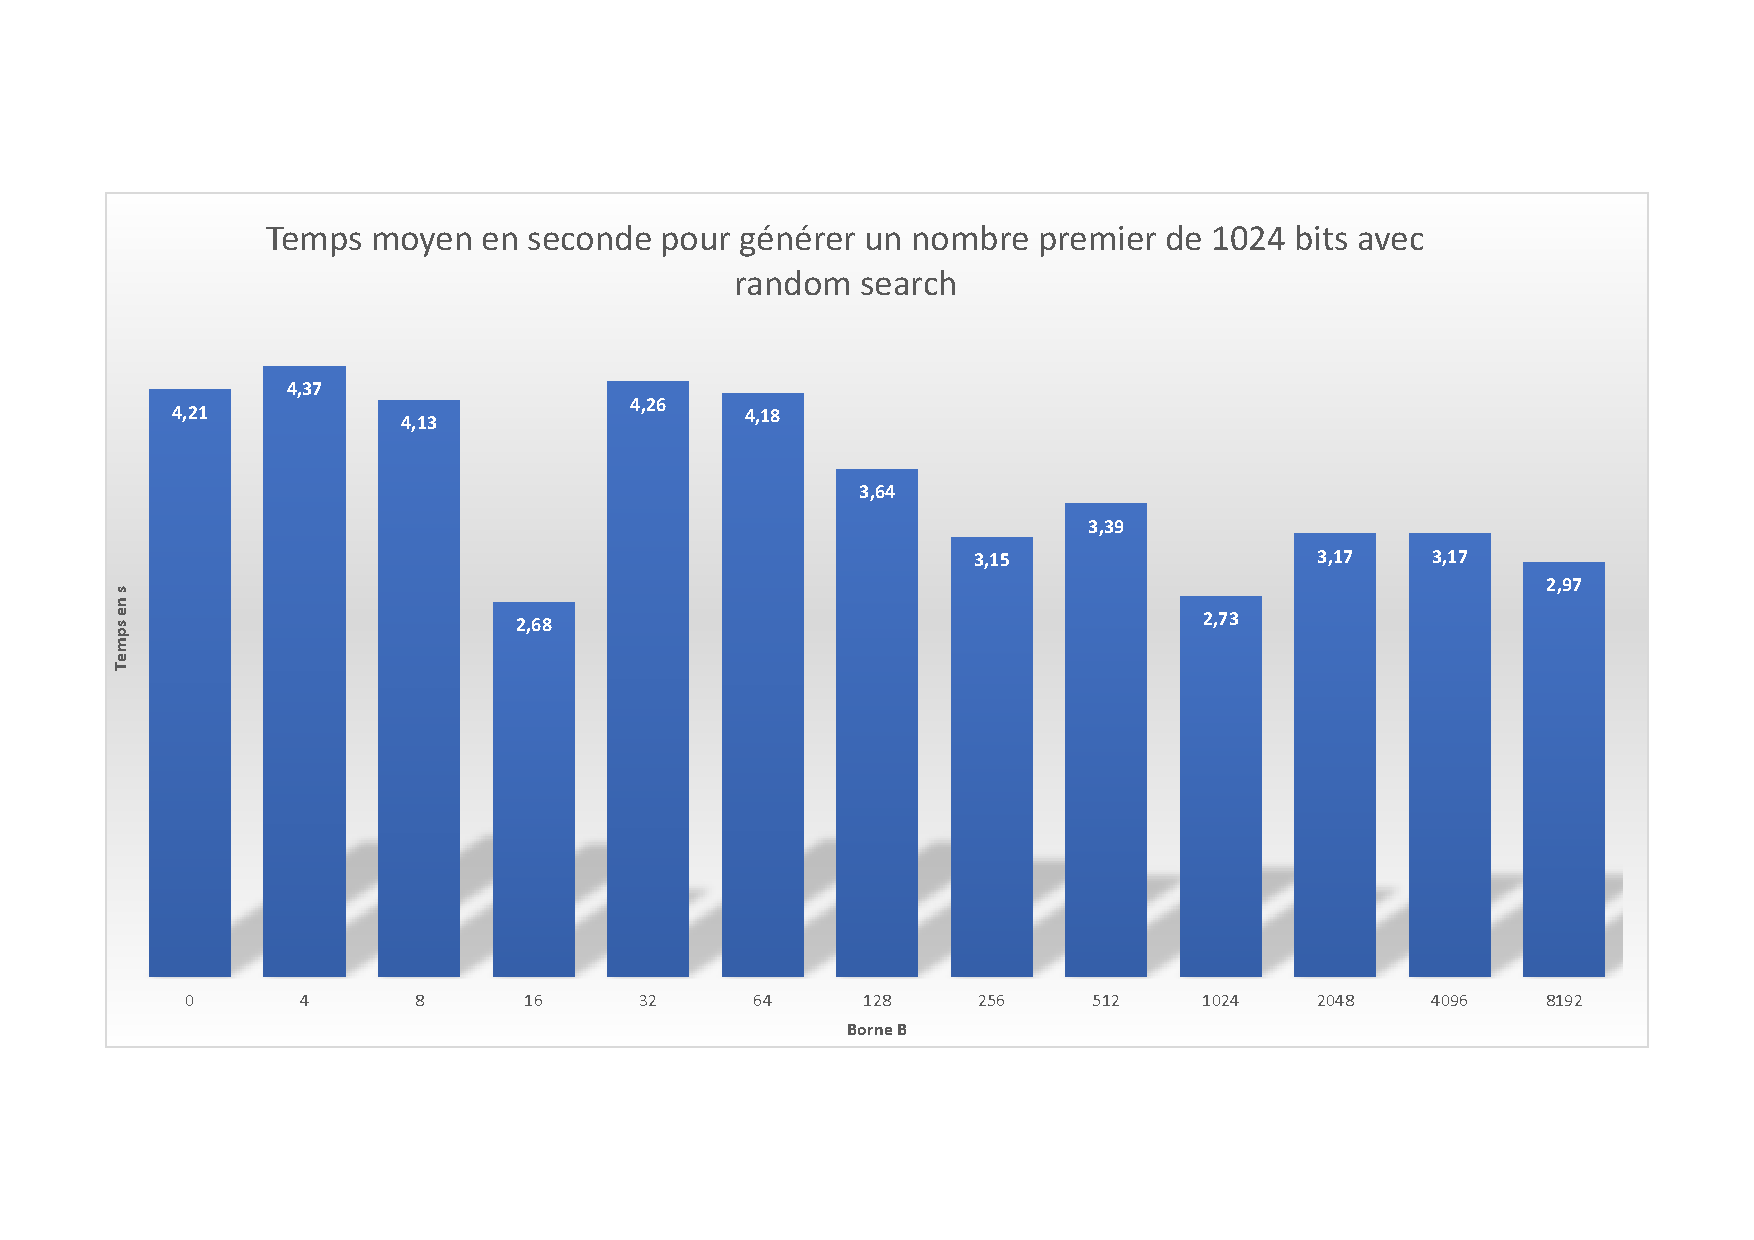
\includegraphics[scale=0.6]{Figures/Graphique.pdf}
    \caption{Graphique moyenne en seconde sur $100$ tests. }
\end{figure}

Voici un graphique récapitulant les tests menés pour générer un nombre premier de $1024$ bits avec RandomSearch et diffèrente valeur de B.
Il semblerait que la valeur optimale pour B spécifique à notre implémentation soit B=16. 

\subsubsection{Choix du paramètre de sécurité t}

Voici le tableau récapitulant les valeurs de $t$ en fonction de la taille du nombre premier a générer pour satisfaire la sécurité décrite \ref{Test probabiliste de primalité}. Ces résultat sont tirés du livre \cite{HAC}.

\begin{figure}[H]
    \centering
    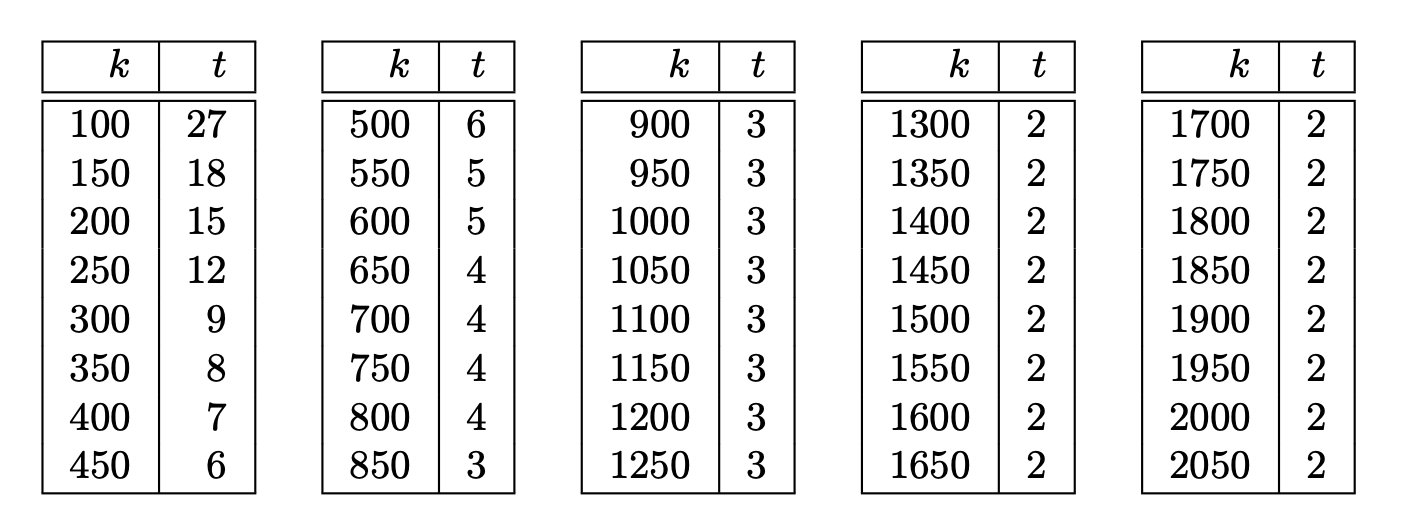
\includegraphics[scale=0.6]{Figures/parametret.png}
    \caption{Tableau des choix de $t$ en fonction de la taille du nombre premier a générer garantissant la sécurité demandée.}
\end{figure}

\section{Algorithme de Gordon}
\label{Algorithme de Gordon}
Le cryptosystème RSA utilise un nombre $n = pq$, où $p$ et $q$ sont des nombres premiers impairs. Les nombres premiers $p$ et $q$ doivent être d’une taille suffisante pour que la factorisation de leur produit soit hors de portée informatique donc d'une recherche exhaustive. La découverte du système cryptographique RSA a conduit à l’étude de contraintes sur le choix de $p$ et $q$ qui est nécessaire pour assurer que le système RSA soit à l’abri des attaques, ainsi la notion d’un premier fort a été définie. Actuellement la meilleure attaque connue est de l'ordre de 712 bits pour casser le système. De nos jours, la notion de nombre premier fort n'est pas forcément utilisé dans tous les systèmes car générer des nombres de 2048 bits est hors de portée d'attaque. Enfin, un nombre premier de 2048 bits peut-être généré par RandomSearch ou Gordon et il faut savoir qu'une clé n'est pas générer tous les jours elle est utilisée assez longtemps. Définissons quand même la notion de nombre premier fort pour la suite et l'utilisation de l'algorithme de Gordon.
\subsection{Nombre premier fort}

Les \textbf{nombres premiers forts} sont utilisés pour générer les clés de codage en cryptographie RSA. Ces nombres créent des cas de résolution impossibles pour ceux qui chercheraient à factoriser les clés du code.

\underline{\textbf{Définition:}}

Un nombre premier est dit \textbf{nombre premier fort} si les entiers r,s et t existent et si les conditions suivantes sont satisfaites:

\begin{enumerate}[label=\arabic*)]
 \item   $ p-1$ à un grand facteur premier noté $r$
 \item   $ p+1$ à un grand facteur premier noté $s$
 \item  $r-1$ à un grand facteur premier noté $t$
\end{enumerate}


Si on prend un exemple, $71$ est un nombre premier fort car il satisfait les conditions ci-dessus. En effet $p=71$, $71=7*10+1$ de plus $7=2*3+1$ et $71=36*2-1$. 

Un nombre premier fort générer pour RSA doit être beaucoup plus grand que cet exemple. Par exemple des nombres de 1024 ou 2048 bits.

\subsection{Algorithme de Gordon et complexité}

Voici l'algorithme de Gordon qui permet de générer un nombre premier fort.

\begin{algorithm}
\caption{Gordon(nbits,$k=20$,$i_0=1$, $j_0=1$)}
\begin{algorithmic}[1]
\Require{Un entier nbits qui définit le nombre de bits }
\Ensure{un entier $p$ de nbits-bit}
\State \textbf{Générer} 2 grand nombres premiers $s$ et $t$ avec $RandomSearch(nbits,k)$
\State  \textbf{Choisir} un entier $i_0$. \textbf{Trouver} le premier nombre premier dans la séquence $2it+1$ pour $i=i_0,i_0+1,i_0=2,...$. \textbf{Noter} ce nombre premier $r=2it+1$
\State \textbf{Calculer} $p_0=2(s^{r-2} \mod r)s -1$
\State  \textbf{Choisir} un entier $j_0$. \textbf{Trouver} le premier nombre premier dans la séquence $p_0+2jrs$ pour $j=j_0,j_0+1,j_0+2,...$. \textbf{Noter} ce nombre premier $p=p_0+2jrs$.
\State \Return p
\end{algorithmic}
\end{algorithm}

Pour générer les 2 grands nombres premiers au début de l'algorithme, nous utiliserons l'algorithme de $RandomSearch(k,t)$. De plus, pour trouver le nombre premier $r$ et $p$ dans la séquence définit dans l'algorithme, on peut notamment utiliser le test de $MillerRabin(n,t)$ ou le test de $Pocklington$ notamment à l'étape 2 pour optimiser le temps de calcul.

\underline{\textbf{Complexité}}:

En utilisant le test de Miller-Rabin, le temps attendus par l'algorithme de Gordon pour trouver un nombre premier fort est d'environ $19\%$ plus grand que la complexité en temps trouvée par l'algorithme pour générer des nombres premiers aléatoires.

\subsubsection{Résultats Expérimentaux}

Nous avons codé notre algorithme avec $MillerRabin(n,t)$ pour tester les nombres $r$ et $p$ afin d'avoir un temps d'exécution proche de $RandomSearch(k,t)$. Nous n'avons pas pu finir pour coder l'algorithme avec le test de Pocklington à l'étape 2 car il est certain que ceci optimiserait le temps. 
On a pris un paramètre de sécurité $k=20$ comme cela on peut faire marcher l'algorithme facilement. Si on teste avec 1024 bits, l'algorithme nous retourne un nombre premier fort en environ 8 secondes ce qui n'est pas négligeable sachant toutes les propriétés à vérifier pour nombre premier fort.
Il est quand même plus logique d'utiliser l'algorithme $RandomSearch(k,t)$ qui comme on l'a dit dans l'introduction est plus efficace que l'algorithme de Gordon pour générer un nombre de 2048 bits premiers et nous garantit déjà d'une sécurité maximale.


\section{Algorithme DSA}
\label{Algorithme DSA}
\underline{\textbf{Définition}}:

 Parmi les nombres premiers forts qui sont utilisés pour générer des clés de codage, on trouve aussi les nombres \textbf{DSA} (Nist Digital Signature Algorithm) qui ont la même utilité. Ils ont plusieurs conditions spécifiques. L'algorithme DSA a besoin de deux nombres premiers $p$ et $q$ qui satisfassent les conditions suivantes:


\begin{enumerate}[label=\roman*)]
 \item  Soit un entier $q$ premier de 256 bits tel que,  $2^{255} \leq q \leq 2^{256}$. 
 \item   Soit un entier $p$ premier tel que ,  $2^{L-1} \leq p \leq 2^{L}$ avec $L=2048+64l$ pour $0\leq l \leq 8$,
 \item  $q$ divise $p-1$
\end{enumerate}

Cette algorithme présente donc comment construire les nombres p et q à partir d'une fonction de hachage. La fonction de hachage utilisé est la fonction Sha-2 qui produit des hachés de $256$ bits. 

Sha-2 est une fonction de hachage cryptographique conçue par la \textit{ National Security Agency} des Etats-Unis qui est un standard de traitement de l'information. Elle produit un résultat de 256 bits (32 octets), habituellement représenté par un nombre hexadécimal. Les algorithmes de la famille SHA-2 sont très semblables, il y a essentiellement deux fonctions différentes, SHA-256(utilisé dans l'algorithme) et SHA-512, les autres étant des variantes de l'une ou l'autre. Les fonctions SHA-256 et SHA-512 ont la même structure mais diffèrent par la taille des mots et des blocs utilisés. Cette structure est assez proche de celle de SHA-1, mais un peu plus complexe et en évite certaines faiblesses connues.

Ici, dans l'algorithme la fonction de Hachage sert notamment à produire les nombres premiers $q$ et $p$ grâce aux entiers $s$ et $s+1 \mod 2^g$. Tout d'abord, on convertit $H(s)$ et $H(s+1 \mod 2^g)$ en base 2 et ensuite on fait le "XOR" sur les entiers c'est-à-dire on fait une addition binaire des deux chaînes. Ensuite, pour trouver $q$ on remplace par 1 les bits de poids faible et de poids fort du résultat du XOR. Finalement, le test de primalité de Miller-Rabin assure le fait que $q$ est premier. Pour trouver $p$ on calcule W tel que: 

$W=V_0 + V_1*2^{256} + V_2*2^{512} +...+V_{n-1}*2^{256(n-1)} + (V_n\mod 2^b)2^{256n}$ avec $V_k=H(s+k+j \mod 2^g)$. 

Ensuite, on calcule un entier X de L bits tel que $X=W+2^{L-1}$. Enfin, on calcule $c=X\mod2^q$ et on définit $p=X-(c-1)$. Pour déterminer si $p$ est premier, on calcule la primalité de $p$ en utilisant le test de Miller-Rabin.
L'algorithme DSA renvoie donc les entiers premiers \textbf{p} et \textbf{q}.

\subsection{Algorithme NIST pour générer les nombres premiers DSA}

\begin{algorithm}[h!]
\caption{DSA(l)}
\begin{algorithmic}[1]
\Require{Un entier l, $0\leq l \leq 8$ }
\Ensure{$q$ un entier de 256 bits premier et p un premier de L bits tel que $L=2048+64l$ et $q|p-1$}
\State Calculer $L=2048+64l$ et trouver le reste $(b)$ et le quotient $(n)$ de la division de $L-1$ par 256   
\State \textbf{Répéter les actions suivantes:}
\State Trouver un entier $s$ aléatoire de longueur binaire $ \leq 256$
\State Calculer $U=H(s) \oplus H(s+1 \mod 2^g)$ et former $q$ grâce à $U$ en remplaçant par 1 le bits de poids faible et de poids fort.
\State Calculer MillerRabin($q$,$t$) pour $t\geq18$ jusqu'à que $q$ soit premier sinon on recommence les étapes.
\State Soit $i=0$ et $j=2$
\While { $i < 4096$ }
\For {$k$ \textbf{allant de} 0 \textbf{à} $n$}
\State $V_k=H(s+k+j \mod 2^g)$ 
\State $W=V_0 + V_1*2^{256} + V_2*2^{512} +...+V_{n-1}*2^{256(n-1)} + (V_n\mod 2^b)2^{256n}$ 
\EndFor
\State $X=W+2^{L-1}$
\State Calculer $c=X\mod2^q$ et définir $p=X-(c-1)$
\If{$p\geq2^{L-1}$ }
\State Utiliser MillerRabin($p$,$t$) pour $t\geq5$. 
\State Si p est premier probable alors \Return (p,q)
\EndIf
\State définir $i=i+1$ et $j=j+n+1$
\EndWhile
\State Revenir à l'étape 2
\end{algorithmic}
\end{algorithm}

\subsubsection{Résultats Expérimentaux}

A la base, l'algorithme est présenté avec la fonction de Hachage Sha-1. C'est fonction n'est plus considéré comme sûr contre des adversaires disposant de moyens importants. En 2005, des cryptanalystes ont découvert des attaques sur SHA-1, suggérant que l'algorithme pourrait ne plus être suffisamment sûr pour continuer à l'utiliser dans le futur. En 2010, Sha-1 a été remplacé par la fonction que nous avons décidé d'utiliser: Sha-2.

Prenons par exemple en entrée un entier l=1. L'algorithme $DSA$ renvoie les entiers $p$ de 2048 bits et $q$ de 256 bits en moyenne en 5 secondes. 

\clearpage

\section{Génération de nombre premiers de Sophie Germain}

\underline{\textbf{Définition}}:

Un nombre premier $p$ est appelé \textbf{nombre premier de Sophie Germain} si $2p+1$ est aussi un nombre premier.
Le nombre $2p + 1$, associé à un premier de Sophie Germain est un \textbf{nombre premier sûr} (safe prime).

Exemple: $11$ et $2*11+1 = 23$ sont tous deux premiers.

Une séquence (chaîne de Cunningham)  apparaît lorsque le nombre associé est lui-même un nombre premier de Sophie Germain. Exemple de séquence à cinq termes:

2, 2x2+1 = 5, 2x5+1 = 11, 2x11+1 = 23, 2x23+1 = 47

\underline{\textbf{Remarque}}:

Finalement, en pratique, pour tester si un nombre est de Sophie Germain il faut appliquer la méthode suivante :

Soit $p$ un nombre premier de la forme $p=4k+3$. Alors $p$ est un nombre premier de Sophie Germain si et seulement si le nombre de Mersenne $M_p = 2^{p} - 1$ est un nombre composé dont $2p+1$ est un diviseur. Cette proposition peut être utilisée comme test de primalité et c'est comme cela que l'on peut faire des records de nombres premiers de Sophie Germain.


\subsection{Historique}

Sophie Germain (1776-1831) est une des premières femmes mathématiciennes. Brillante autodidacte, estimée par quelques uns de ses pairs, elle s'est toutefois heurtée à l'intransigeance de son époque envers les femmes savantes.
A 19 ans, elle parvient à obtenir les notes de cours de l'Ecole Polytechnique nouvellement créée. Pour pouvoir se consacrer aux mathématiques, alors réservées aux hommes, elle utilisa un nom d’emprunt de 1794 à 1807 : Antoine Auguste Le Blanc. Elle commence à entretenir une correspondance avec Lagrange, qui y est professeur d'Analyse.

La théorie des nombres est le premier domaine où Sophie Germain apporte une contribution importante. On lui doit notamment les plus importantes avancées sur le théorème de Fermat depuis Euler (1738), et avant Kummer (1840). Elle démontre que si n est un nombre premier (distinct de 2) tel que $2n+1$ est un nombre premier, alors un triplet d'entiers (x,y,z) ne peut vérifier l'équation de Fermat :
\begin{center}
$x^n + y^n = z^n$.
\end{center}
Elle décrit aussi une classe particulière de nombres, devenus les nombres premiers de Sophie Germain. Un nombre est de ce type si son double plus 1 est premier aussi.

A la suite de la visite du physicien allemand Chladni à Paris en 1809, Sophie Germain change radicalement d'orientation mathématique. Pendant plus d'une décennie, elle s'intéressera à la théorie des surfaces (principalement à leur courbure) et au problème de vibration des surfaces élastiques. Sophie Germain continue à travailler jusqu'à la fin de sa vie sur les mathématiques et la philosophie. Elle décède le 27 juin 1831, victime d'un cancer du sein.

